\chapter{Időlépéses megoldó módszerek}\label{chap:idolep_tan} 

{\ }

Az építőmérnöki gyakorlatban használt szerkezeti rendszerek dinamikus terhelésekor  legtöbbször numerikus számítási eljárásokat alkalmazunk. A szerkezeteket térben és időben is diszkretizáljuk. A térbeli diszkretizálás történhet például végeselem módszerrel, az időbeli diszkretizáláshoz pedig időlépéses integráló formulákat használhatunk.  A dinamikus mozgásegyenlet problémája matematikailag egy közönséges differenciálegyenlet kezdetiérték-feladat, melyre számos matematikai eljárást dolgoztak ki, többet kifejezetten építőmérnöki alkalmazásra. A legfontosabb lineáris és nemlineáris módszereket ismertetem dolgozatomban. 

Az időlépéses megoldó módszerek alkalmazásakor diszkrét időpontokban oldjuk meg a \eqref{rezgesegy} mátrix-differenciálegyenletet. Elöljáróban bevezetünk néhány jelölést. A vizsgált időpontokat $t_i$-vel jelöljük, ahol $i = 0,1,...,N-1$. Két időpont között definiáljuk  a lépésközt:
%
\begin{equation*}
t_{i+1}-t_i  = \Delta{t}  
\end{equation*}
Csak olyan eseteket fogunk vizsgálni, amikor $\Delta{t} = konstans$ és $t_i = i\Delta{t}$.

A $t_i$ időpontokhoz tartozó állapotjellemzőkre bevezethetjük a következő rövidített jelöléseket:
%
\begin{align*} 
\label{eq:u_i}
\mathbf{u}_i & = \mathbf{u}(t_i),  & \mathbf{\dot{u}}_i & = \mathbf{\dot{u}}(t_i),  \\
\mathbf{\ddot{u}}_i & = \mathbf{\ddot{u}}(t_i),  & \mathbf{q}_i & = \mathbf{q}(t_i) \\
\mathbf{f}_{s}(\mathbf{u}_{i}) & = \mathbf{f}_{s,i}. 
\end{align*}
%
A $t_i$ időpontban a \eqref{rezgesegy} alatti lineáris mátrix-differenciálegyenlet ezek behelyettesítésével:
%
\begin{equation}
\label{rezgegyi}
\mathbf{M}\mathbf{\ddot{u}}_i+\mathbf{C}\mathbf{\dot{u}}_i+\mathbf{K}\mathbf{u}_i = \mathbf{q}_{i}.
\end{equation}
%
A \eqref{rezgesegy_nemlin} nemlineáris mátrix-differenciálegyenletet  ezeket a jelöléseket használva  $t_i$ időpontban a következőképp írhatjuk fel:
%
\begin{equation}
\label{rezgegyi_nl}
\mathbf{M}\mathbf{\ddot{u}}_i+\mathbf{C}\mathbf{\dot{u}}_i+\mathbf{f}_{s,i} = \mathbf{q}_{i}.
\end{equation}
%
A $t_{i+1}$ időponthoz tartozó állapotjellemzőket a következőképpen jelölhetjük:
%
\begin{align*} 
\label{eq:u_i1}
\mathbf{u}_{i+1} & = \mathbf{u}(t_{i+1}),  & \mathbf{\dot{u}}_{i+1} & = \mathbf{\dot{u}}(t_{i+1}),  \\
\mathbf{\ddot{u}}_{i+1} & = \mathbf{\ddot{u}}(t_{i+1}),  & \mathbf{q}_{i+1} & = \mathbf{q}(t_{i+1}) \\
\mathbf{f}_{s}(\mathbf{u}_{i+1}) & = \mathbf{f}_{s,i+1}. 
\end{align*}
%
Ezeket behelyettesítve, a $t_{i+1}$ időpontban felírva a \eqref{rezgesegy} lineáris egyenletet:
%
\begin{equation}
\label{rezgegyi+1}
\mathbf{M}\mathbf{\ddot{u}}_{i+1}+\mathbf{C}\mathbf{\dot{u}}_{i+1}+\mathbf{K}\mathbf{u}_{i+1}=\mathbf{q}_{i+1}.
\end{equation}
%
A  \eqref{rezgesegy_nemlin} nemlineáris differenciálegyenlet pedig a következőképp alakul:
%
\begin{equation}
\label{rezgegyi+1_nl}
\mathbf{M}\mathbf{\ddot{u}}_{i+1}+\mathbf{C}\mathbf{\dot{u}}_{i+1}+\mathbf{f}_{s,i+1}=\mathbf{q}_{i+1}.
\end{equation}

A továbbiakban a bevezetett jelöléseket és a  \eqref{rezgegyi}, \eqref{rezgegyi_nl}, \eqref{rezgegyi+1}, valamint \eqref{rezgegyi+1_nl} differenciálegyenleteket használjuk. 


\section{Időlépéses módszerek általános ismertetése}

%A módszerek stabilitásának és pontosságának elemzése legegyszerűbben az egyszabadságfokú rendszerek szabad rezgésének vizsgálatával végezhető.

{\ }

A vizsgált rendszerek alapján a feladat lehet lineáris, amit az \eqref{rezgesegy} egyenlet ír le, és nemlineáris ami az \eqref{rezgesegy_nemlin} egyenlettel jellemezhető. A lineáris feladatokra jellemző, hogy sokkal egyszerűbb eljárások alkalmazhatók, és ezek könnyebben is programozhatók. Azonban, mivel a linearitás általában csak egyszerűsítő feltételezés a vizsgált rendszer leírására, a nemlineáris egyenlet megoldása pontosabb közelítést ad a valós szerkezeti viselkedésre.

Az időlépéses módszerek jellemzésére különböző szempontokat alkalmazunk. Megkülönböztetünk explicit és implicit eljárásokat, illetve vizsgálhatjuk az eljárások stabilitását és pontosságát is.

\subsection{Az időlépéses módszerek jellemzése}

{\ }

A numerikus eljárások két csoportra oszthatók \cite{gyorgyi}. Explicit eljárásról beszélünk, ha a $t_{i+1}$ időponthoz tartozó elmozdulások  a $t_i$ időpontban felírt dinamikai egyenletekből meghatározhatók. Az implicit eljárásnál viszont a $t_{i+1}$ időponthoz tartozó elmozdulás meghatározásához a mátrix-differenciálegyenletet a $t_{i+1}$ időpontban kell kielégíteni.

Az explicit eljárások egyszerűbbek és könnyebben programozhatók, viszont hátrányuk, hogy kisebb $\Delta{t}$ integrálási időközre van szükség. Az implicit eljárások esetében az egyes időlépések alatt iterációs számítás történik, ezért nagyobb $\Delta{t}$ lépésköz engedhető meg, viszont így az algoritmus bonyolultabb és nehezebben programozható.

Az eljárásoktól elvárjuk, hogy stabilak és megfelelően pontosak legyenek. 

A módszerek stabilitása azt jelenti, hogy számítás során az amplitúdók nem növekednek korlátlanul (nem tartanak a végtelenbe). Egy eljárás feltétel nélkül stabil, ha bizonyos beállításokkal a módszer stabilitása nem függ $\Delta{t}$ lépésköz nagyságától, és feltételesen stabil, ha az eljárás stabilitása $\Delta{t}$ megfelelő megválasztásától függ.

Általában az implicit eljárások esetében beszélhetünk feltétel nélküli stabilitásról, és az explicit eljárások feltételesen stabilak. Ez alól kivétel az explicit Chen-Ricles  algoritmus, mely a megfelelő paraméterek megválasztásával feltétel nélkül stabil.

A stabilitás biztosítása azonban nem jelenti az eljárás pontosságát is. Különösen fontos ezt a feltétel nélkül stabil eljárásoknál kiemelni.  Az eljárások pontossága azt jelenti, hogy megfelelő hibahatáron belüli közelítést adnak a valós megoldásra.

Általános esetben a megoldás a sajátrezgésalakokhoz tartozó harmonikus rezgések összegzéseként adódik. Ha egy rezgésalak változását ábrázolni akarjuk, akkor egy ökölszabály szerint a hozzátartozó periódusidőt  legalább tíz részre kell osztani ahhoz, hogy a rezgés  harmonikusnak látszódjon. Ebből a megfontolásból kiindulva azt mondhatjuk, hogy a $\Delta{t}$ időlépés a még számításba veendő legmagasabb sajátkörfrekvenciájú rezgés periódusidejének megfelelően, legfeljebb 
%
\begin{equation}
\label{dt max}
\Delta{t} = \frac{T_m}{10}
\end{equation}
% 
értéket veheti fel. 



A modell pontosságából azonban még nem következik az eljárás pontossága. Az ugyanis akkor is kérdéses, ha minden rezgésalak szerepel a megoldásban, és a lépésközt a \eqref{dt max}-nek megfelelően választjuk meg. A numerikus integrálásnál kétféle hibával találkozhatunk. Az egyik hiba a periódus idő meghosszabbodása (Period Elongation, PE), a másik hiba pedig az amplitúdó csökkenése (Amplitude Decay, AD). A \ref{fig:pont} ábrán egy csillapítatlan harmonikus rezgés pontatlanságai láthatók.

  \begin{figure}[h!]
\centering
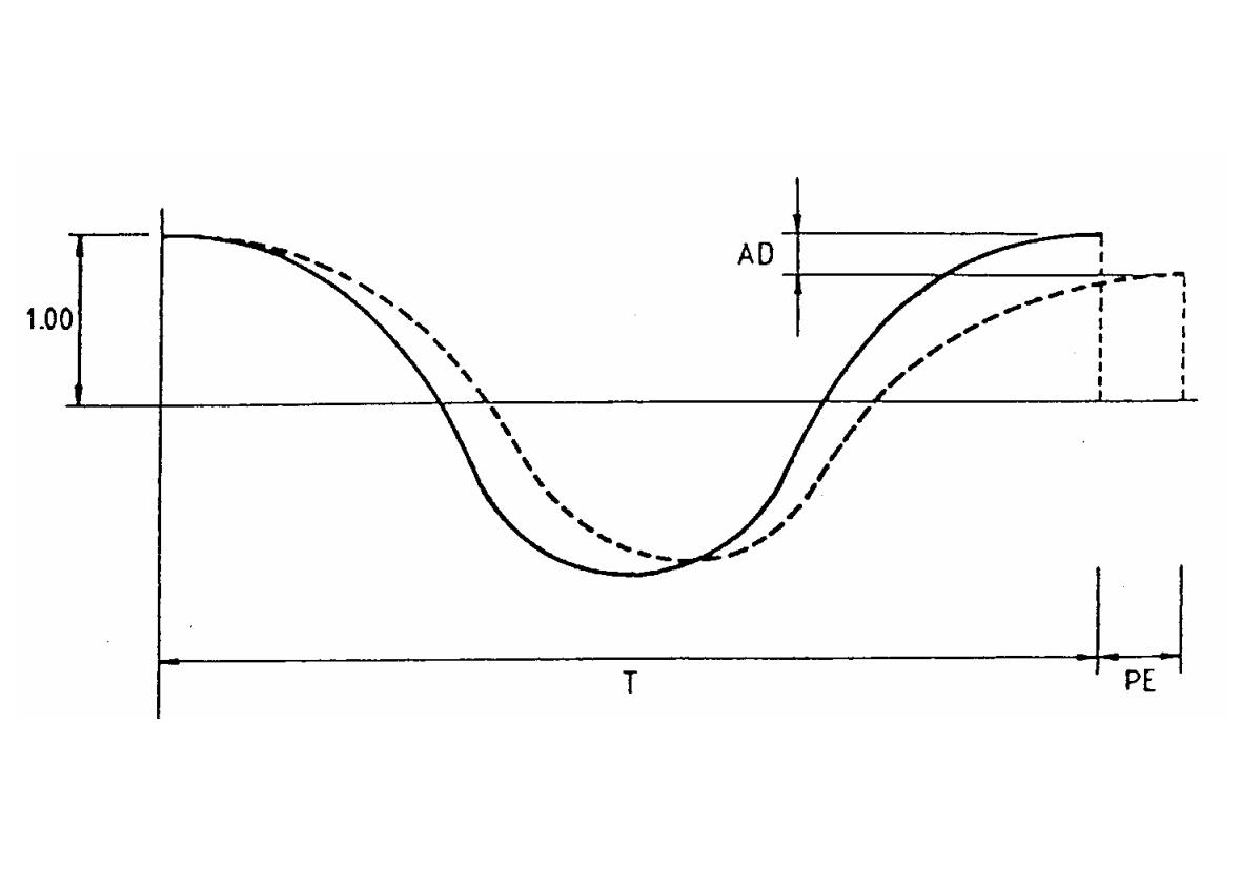
\includegraphics[width=0.75\textwidth]{pontatlansag.pdf}
\caption{A numerikus integrálás pontatlanságai \cite{gyorgyi}.}
\label{fig:pont}
\end{figure}
 
Az ábrán "T" a periódusidőt jelenti. A folytonos vonal a valós elmozdulást, a szaggatott pedig a numerikus számításból adódó elmozdulást  jelöli.


\subsection{Időlépéses módszerek stabilitásának vizsgálata}

{\ }

A numerikus számításoktól elvárjuk, hogy stabilak legyenek. A stabilitás csillapítatlan szabadrezgés esetén szemléltethető a legjobban. Az  integráló formulát akkor tekinthetjük stabilnak, ha a rendszer beáll valamilyen állandósult rezgésre. Ha  azonban a megoldás azt eredményezi, hogy a rendszerben egyre növekvő elmozdulások keletkeznek, az integráló eljárás az adott paraméterekkel nem nevezhető stabilnak. A követezőkben bemutatom az általános stabilitásvizsgálatot.

Először definiáljuk $t_i$ és $t_{i+1}$ időpontpeli mozgásjellemzőket a következő vektorokkal:
\begin{align*}
\mathbf{\hat{u}}_i & = \left[ \begin{array}{cc} \mathbf{u}_i \\ \mathbf{\dot{u}}_i \end{array} \right], & \mathbf{\hat{u}}_{i+1} & = \left[ \begin{array}{cc} \mathbf{u}_{i+1} \\ \mathbf{\dot{u}}_{i+1} \end{array} \right].
\end{align*}
Minden eljárás esetében felírható egy általános összefüggés a $t_{i+1}$ és $t_i$ időpontbeli mozgásjellemzők között:
\begin{equation}
\label{stab}
\mathbf{\hat{u}}_{i+1} = \mathbf{A}\mathbf{\hat{u}}_i.
\end{equation}
Ekkor az $\mathbf{\hat{u}}_t$ vektorban a $t+\Delta{t}$ időponthoz tartozó érték számításához szükséges jellemzők szerepelnek. A kifejezés felírható a következő alakban:
\begin{equation*}
\mathbf{\hat{u}}_{n} = \mathbf{A}\mathbf{\hat{u}}_{n-1} = \mathbf{A}^{n}\mathbf{\hat{u}}_1.
\end{equation*}
Az $\mathbf{A}^n$ mátrix felírható
\begin{equation*}
\mathbf{A}^n = \mathbf{P}\mathbf{J}^n\mathbf{P}^{-1},
\end{equation*}
alakban, ahol a $\mathbf{P}$ mátrixban az $\mathbf{A}$ mátrix sajátvektorai, a $\mathbf{J}$ mátrix főátlójában pedig az $\mathbf{A}$ mátrix sajátértékei helyezkednek el. A kifejezés stabilitásának feltétele, hogy az $\mathbf{A}^n$ mátrix ne a végtelenhez konvergáljon, tehát a sajátértékek  abszolút értéke maximum 1 legyen:
\begin{equation}
\rho\left(\mathbf{A}\right) = max|\lambda_k| \leq 1.
\label{stab felt}
\end{equation}  

A \eqref{stab felt} kifejezést az egyes eljárások esetében megoldva definiálhatjuk a feltételes és a feltétel nélküli stabilitást. Ha azt kapjuk eredményül, hogy az integrálási lépésköz frekvenciafüggő, akkor feltételes stabilitásról beszélhetünk. Ez többnyire az explicit eljárásokra jellemző. Amikor viszont a stabilitási vizsgálatot elvégezve az eredmény nem függ a sajátkörfrekvenciától, az eljárást feltétel nélkül stabilnak nevezzük. Ezeknél az eljárásoknál a stabilitás valamilyen integrálási paraméter függvénye. Többnyire ebbe a csoportba  az implicit módszerek tartoznak. Kivételt képez a Chen-Ricles algoritmus, ami egy feltétel nélkül stabil explicit eljárás.  


\subsection{Időlépéses módszerek alkalmazása modálanalízis esetén}

{\ }

Nagyméretű feladatok esetén előfordulhat olyan eset, hogy a modálanalízis és a numerikus integrálás együttes alkalmazása válik szükségessé \cite{gyorgyi}. 

Arányos csillapítás esetén az ekvivalens csillapítási mátrix felírható formális alakban:
\begin{equation}
\label{csill}
\mathbf{C} = \frac{\gamma}{\omega_{0r}}\mathbf{K},
\end{equation}
ahol $\omega_{0r}$ az $r$-edik sajátkörfrekvencia. A \eqref{csill} kifejezést formálisan behelyettesítve a \eqref{rezgegy} mátrix-differenciálegyenletbe:
\begin{equation*}
\mathbf{M}\mathbf{\ddot{x}}(t)+\frac{\gamma}{\omega_{0r}}\mathbf{K}\mathbf{\dot{x}}(t)+\mathbf{K}\mathbf{x}(t) = \mathbf{p}(t).
\end{equation*}
Ilyenkor a feladat csak modálanalízis és numerikus integrálás együttes alkalmazásával kezelhető.

Bevezetve az $\mathbf{x} = \mathbf{V}\mathbf{y}(t)$ összefüggést, ahol $\mathbf{V}$ a sajátvektorok mátrixa, és megszorozva az egyenletet balról $
\mathbf{V}^T$ mátrixszal az alábbi egyenletet kapjuk:
%
\begin{equation*}
\mathbf{V}^T\mathbf{M}\mathbf{V}\mathbf{\ddot{y}}(t)+\frac{\gamma}{\omega_{0r}}\mathbf{V}^T\mathbf{K}\mathbf{V}\mathbf{\dot{y}}(t)+\mathbf{V}^T\mathbf{K}\mathbf{V}\mathbf{y}(t) = \mathbf{V}^T\mathbf{q}(t)
\end{equation*}
%
Ekkor a mátrix-differenciálegyenlet n számú független egyszabadságfokú rezgés differenciálegyenletére esik szét:
%
\begin{equation*}
\ddot{y}_r(t)+\gamma\omega_{0r}\dot{y}_r(t)+\omega_{0r}^2y_r(t) = \mathbf{v_r}^T\mathbf{q}(t) = f_r(t),
\end{equation*}
%
ahol $f_r(t)$ az idő tetszőleges függvénye. Egyszabadságfokú rendszerre is alkalmazhatók a numerikus integráló eljárások. A számítás $t = 0$ időpontban kezdődik. Az ehhez tartozó kezdeti feltételek:
\begin{align*}
%
y_{0r} & = \mathbf{v}_r^T\mathbf{M}\mathbf{x}_0, & \dot{y}_{0r} =  \mathbf{v}_r^T\mathbf{M}\mathbf{\dot{x}}_0,
\end{align*}
%
és $\ddot{y}_{0r}$ értékek az
%
\begin{equation*}
\ddot{y}_{0r}+\gamma\omega_{0r}\dot{y}_{0r}+\omega_{0r}^2y_{0r} =  f_r(0)
\end{equation*}
%
egyenletből számíthatók. Az egyes időlépésekben az $y_r(t_{i+1}) = y_{r,i+1}$ értékeket kiszámítva az elmozdulásvektor a sajátvektorok segítségével:
%
\begin{equation*}
\mathbf{u}_{i+1} = \sum_{r=1}^{n}\mathbf{v}_r{y}_{r,i+1}.
\end{equation*}

%Fontos kérdés modálanalízis nagyméretű feladatokra alkalmazásánál, hogy mennyi sajátvektort kell figyelembe venni.


\section{Időlépéses módszerek alkalmazása lineáris rendszerek vizsgálatára}\label{sec:idolepmsz}

{\ }

A lineáris  szerkezetek viselkedése jól ismert a különböző hatásokra, mozgásegyenleteik pedig a nemlineáris mozgásegyenletekhez képest jóval egyszerűbbek. Számos numerikus integráló eljárást fejlesztettek lineáris egyenletek megoldására. A következőkben a legfontosabb lineáris  módszereket ismertetem.

\subsection{Euler-Cauchy módszer}

{\ }

Az Euler-Cauchy-, vagy más néven explicit Euler-módszer \cite{nummat}, az elmozdulás görbéjét a $t_i$ és $t_{i+1}$ időpontok között a görbe $t_i$ pontbeli érintőjével közelíti. A módszert  szokás töröttvonalmódszernek is nevezni.

A sebesség függvénye felírható és átalakítható az alábbi módon:
\begin{align*}
\mathbf{\dot{u}}(t) & = f(\mathbf{u}), \\
\frac{d\mathbf{u}(t)}{dt} & = f(\mathbf{u}), \\
d\mathbf{u} & = f(\mathbf{u})dt.
\end{align*}
Az időbeni diszkretizálást követően  a sebesség változása a $\Delta{t}$ intervallumon, a $\Delta{t}$-ben magasabb rendű tagokat elhanyagolva:
\begin{equation}
\label{euler du}
\Delta{\mathbf{u}} = \Delta{t}f(\mathbf{u}).
\end{equation}
A \eqref{euler du} kifejezést felhasználva az elmozdulás a $t_{i+1}$ időpontban:
\begin{equation}
\label{euler ui1}
\mathbf{u}_{i+1}  = \mathbf{u}_i+\Delta{\mathbf{u}}_i,  = \mathbf{u}_i+\Delta{t}\mathbf{\dot{u}}_i.
\end{equation}

A \eqref{euler ui1} kifejezésből látszik, hogy a módszer explicit, mert a $t_i$ időpontbeli értékek ismeretében közvetlenül meghatározhatók a $t_{i+1}$ pontbeli közelítések. 

Az eljárás nem stabil, a közelítésnél egyre nagyobb hibák fognak adódni. A lokális hiba $t^2$-tel arányos.


\subsection{Runge-Kutta típusú módszerek}

{\ }

A Runge-Kutta típusú módszerek \cite{nummat} az egylépéses explicit Euler- módszer "finomításának" mondhatók. Az elmozdulás görbéjét a $t_i$ és $t_{i+1}$ pontok közötti osztópontokba húzott érintőkkel közelítjük, tehát egy időlépés alatt több lépésben számítjuk az elmozdulásgörbét.

A másodrendű módszerek (röviden RK2) közül a legegyszerűbb a javított explicit Euler-módszer: a $t = t_{i}+0.5\Delta{t} = t_{i+0.5}$ felezőpontban explicit Euler-módszerrel kiszámoljuk az $\mathbf{u}(t)$ pontos érték $\mathbf{u}_{i+0.5} = \mathbf{u}_i+0.5\Delta{t}\mathbf{\dot{u}}_i$ közelítését, majd ezzel az értékkel meghatározott irányban egy újabb explicit Euler-módszert írunk fel a teljes intervallumra. Az elmozdulás $t_{i+1}$ időpontban ekkor:
\begin{equation*}
\mathbf{u}_{i+1} = \mathbf{u}_i+ \Delta{t}\mathbf{\dot{u}}_{i+0.5}.
\end{equation*}
A lokális hiba RK2 módszernél $t^3$-nal arányos.

 A harmadrendű módszerek közül  (röviden RK3) az egyik módszer esetén $t = t_{i}+0.3\Delta{t} = t_{i+0.3}$ és $t = t_{i}+0.6\Delta{t} = t_{i+0.6}$ harmadolópontokban határozzuk meg a közelítő érintőket. Ebből a $t_{i+1}$ időpontra az elmozdulás:
\begin{equation*}
\mathbf{u}_{i+1} = \mathbf{u}_i+0.5\Delta{t}\mathbf{\dot{u}}_{i+0.3}+0.5\Delta{t}\mathbf{\dot{u}}_{i+0.6}.
\end{equation*}
A lokális hiba ekkor $t^4$-nel arányos.

Felírhatók magasabb rendű Runge-Kutta módszerek is. Minél magasabb rendű az alkalmazott módszer, annál pontosabb eredményt kaphatunk, viszont egy időlépés alatt annál több közbenső lépést kell kiszámolnunk. A gyakorlatban ezért általában a negyed- és ötödrendű módszer a legmagasabb, ami előfordulhat. Léteznek a programrendszerekben olyan beépített programok, amik  beágyazott módszereket alkalmaznak. Ezek lényege, hogy  kiszámolnak két különböző rendű Runge-Kutta módszert (pl. egy negyed- és egy ötödrendűt), és úgy választanak lépésközt, hogy a hiba az alacsonyabb rendű hibája legyen.

\subsection{Centrális differenciák módszere}

{\ }

A centrális differenciák módszerében \cite{gyorgyi} az elmozdulásvektorok függvényét a $t_{i-1}, t_i$ és $t_{i+1}$ időpontokhoz tartozó $\mathbf{u}_{i-1}, \mathbf{u}_i, \mathbf{u}_{i+1}$ vektorelemek értékein átmenő másodfokú parabolákkal közelítjük (lásd: \ref{fig:centdiff} ábra). Ekkor:
%
\begin{align*}
\label{centdiff_av}
\mathbf{\dot{u}}_i&=\frac{1}{2\Delta{t}}\left(\mathbf{u}_{i+1}-\mathbf{u}_{i-1}\right), \\
\mathbf{\ddot{u}}_i&=\frac{1}{\Delta{t}^2}\left(\mathbf{u}_{i+1}-2\mathbf{u}_i+\mathbf{u}_{i-1}\right).
\end{align*}
%
A differenciahányadosokat behelyettesítve a \eqref{rezgegyi} alatti mátrix-differenciálegyenletbe $\mathbf{u}_{i+1}$-re az alábbi összefüggést kapjuk:
%
\begin{equation}
\label{centdiff long}
\left(\frac{1}{\Delta{t}^2}\mathbf{M}+\frac{1}{2\Delta{t}}\mathbf{C}\right)\mathbf{u}_{i+1} = \mathbf{q}_{i}+\left(\frac{2}{\Delta{t}^2}\mathbf{M}- \mathbf{K}\right)\mathbf{u}_i+\left(\frac{1}{2\Delta{t}}\mathbf{C}-\frac{1}{\Delta{t}^2}\mathbf{M}\right)\mathbf{u}_{i-1}.
\end{equation}
%
Az egyenlet rövidebb alakban a következőképp írható fel:
\begin{equation}
\label{centdiff short}
\mathbf{\hat{M}}\mathbf{u}_{i+1} = \mathbf{\hat{q}}_i,
\end{equation}
%
ahol $\mathbf{\hat{M}}$ a hatékony tömegmátrix, $\mathbf{\hat{q}}_i$ pedig a hatékony tehervektor $t_i$ időpillanatban. A módszer az explicit eljárások közé tartozik.

\begin{figure}[h!]
\centering
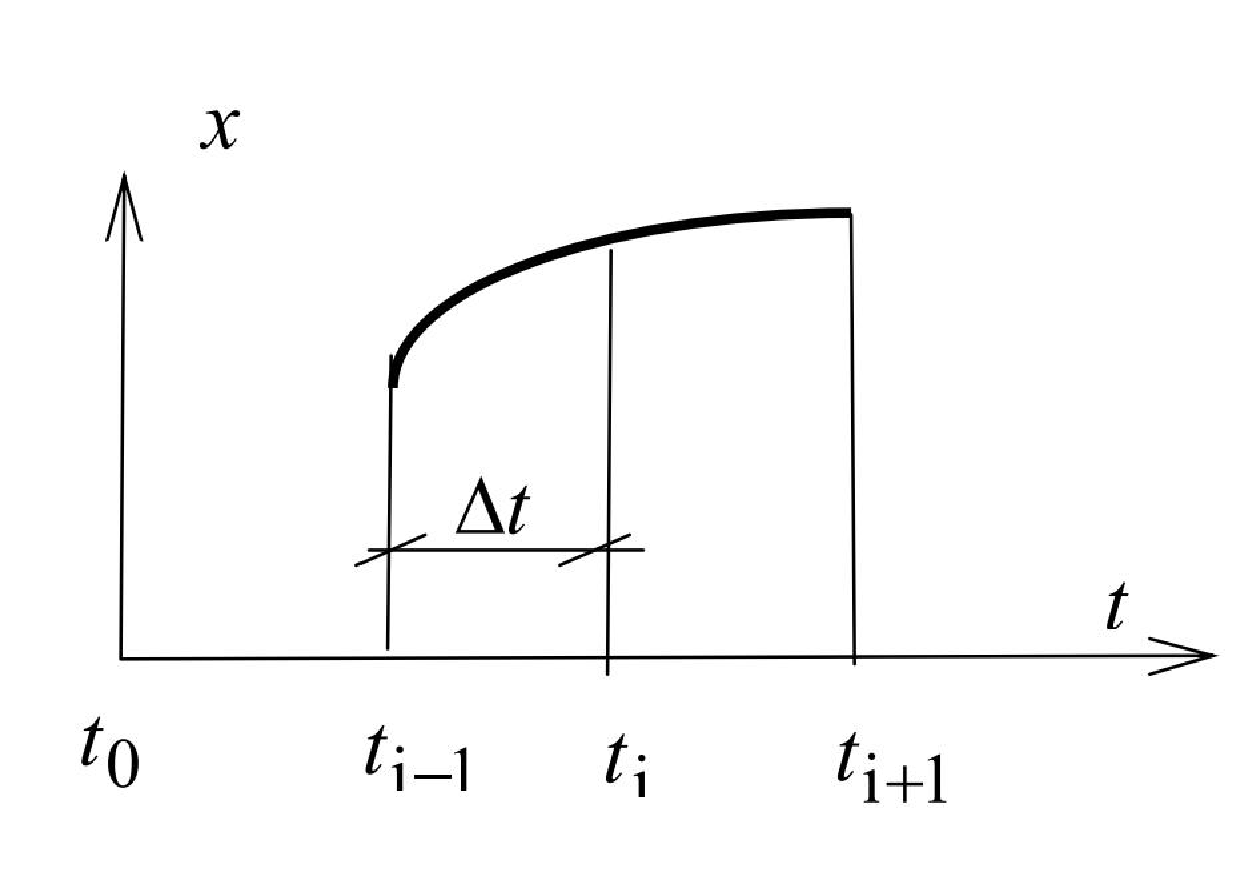
\includegraphics[width=0.5\textwidth]{centdiff.pdf}
\caption{Közelítő elmozdulások a centrális differenciák módszere szerint \cite{gyorgyi}.}
\label{fig:centdiff}
\end{figure}

Adott időpontban az elmozdulás kiszámításához mindig szükség van a megelőző két időpontbeli elmozdulásra, viszont a sebesség és elmozdulásvektorokat nem kell kiszámolni, ezeknek csak a kezdeti időpontbeli értékét használjuk. Az $\mathbf{u}_1$ vektor számításakor az $\mathbf{u}_{i-1}=\mathbf{u}_{-1}$ vektor helyére az
\begin{displaymath}
\label{u_min1}
\mathbf{u}_{-1}=\frac{(\Delta{t})^2}{2}\mathbf{\ddot{u}}_0-\Delta{t}\mathbf{\dot{u}}_0+\mathbf{u}_0
\end{displaymath}
%
összefüggés írható.

A eljárás feltételesen stabil, a szükséges időlépés frekvenciafüggő. A stabilitás feltétele:
\begin{equation*}
\Delta{t} \leq \frac{T_m}{\pi} = \frac{2}{\omega_0}.
\end{equation*}


\subsection{Newmark eljárás}\label{subsec:Newmark_lin}

{\ }

A Newmark eljárás \cite{gyorgyi} a $t_i$ és $t_{i+1}$ időpontok között egy $f(\tau)$ függvény szerinti gyorsulásváltozást feltételez. A gyorsulás ekkor a két időpont között egy $t_i+\tau = t_{i+\tau}$ időpontban:
\begin{equation*}
\mathbf{\ddot{u}}_{i+\tau} = \mathbf{\ddot{u}}_i+f(\tau)(\mathbf{\ddot{u}}_{i+1}-\mathbf{\ddot{u}}_i).
\end{equation*}
Az $f(\tau)$ értéke $\tau = 0$-nál zérus, míg $\tau = \Delta{t}$-nél 1. Az $f(\tau)$ függvénynek az eljárás stabilitásában van szerepe, és a továbbiakban $\gamma = \frac{1}{\Delta{t}}\int_0^{\Delta{t}}f(\tau)d\tau$ és $\beta = \frac{1}{\Delta{t}^2}\int_0^{\Delta{t}}\int_0^{\tau}f(\tau)d\tau$ paraméterekkel jellemezzük. 

Ezek után  a sebesség és gyorsulásvektor $\tau = \Delta{t}$ esetén a $t_{i+1}$ időpontban:
%
\begin{subequations}
\begin{align}
\mathbf{\dot{u}}_{i+1}& =  \mathbf{\dot{u}}_i+[(1-\gamma)\Delta{t}]\mathbf{\ddot{u}}_i+(\gamma\Delta{t})\mathbf{\ddot{u}}_{i+1},   \label{newmark1}\\ 
\mathbf{u}_{i+1}& =  \mathbf{u}_i+\Delta{t}\mathbf{\dot{u}}_i+\left[(0.5-\beta)
(\Delta{t})^2\right]\mathbf{\ddot{u}}_i+\left[\beta(\Delta{t})^2\right]\mathbf{\ddot{u}}_{i+1}. \label{newmark2}
\end{align}
\end{subequations}
% 
Ezeket behelyettesítve az \eqref{rezgesegy} alatti mátrix-differenciálegyenletet az i+1-dik időlépésben teljesítő \eqref{rezgegyi+1} egyenletbe, $\mathbf{u}_{i+1}$-re az alábbi összefüggést kapjuk:
%
\begin{equation}
\label{newmark long}
\begin{split}
\left(\mathbf{K}+\frac{1}{\beta\Delta{t}^2}\mathbf{M}+\frac{\gamma}{\beta\Delta{t}}\mathbf{C}\right)\mathbf{u}_{i+1} = \mathbf{q}_{i+1}+\mathbf{M}\left[\frac{1}{\beta\Delta{t}^2}\left(\mathbf{u}_i+\mathbf{\dot{u}}_i\Delta{t}\right)+\left( \frac{1}{2\beta}-1\right)\mathbf{\ddot{u}}_i\right]        \\ +\mathbf{C}\left[\frac{\gamma}{\beta\Delta{t}}\mathbf{u}_i+\left(\frac{\gamma}{\beta}-1\right)\mathbf{\dot{u}}_i+\left(\frac{\gamma}{2\beta}-1\right)\Delta{t}\mathbf{\ddot{u}}_i\right].
\end{split}
\end{equation}
%
Rövidebb alakban:
\begin{equation}
\label{newmark short}
\mathbf{\hat{K}}\mathbf{u}_{i+1} = \mathbf{\hat{q}}_{i+1},
\end{equation}
% 
ahol $\mathbf{\hat{K}}$ a hatékony merevségi mátrix, $\mathbf{\hat{q}}_{i+1}$ pedig a hatékony tehervektor a $t_{i+1}$ időpillanatban. Az együtthatómátrix lineáris szerkezet esetén időben állandó, ekkor a számítását és invertálását elég egyszer elvégezni.

\begin{figure}[h!]
\centering
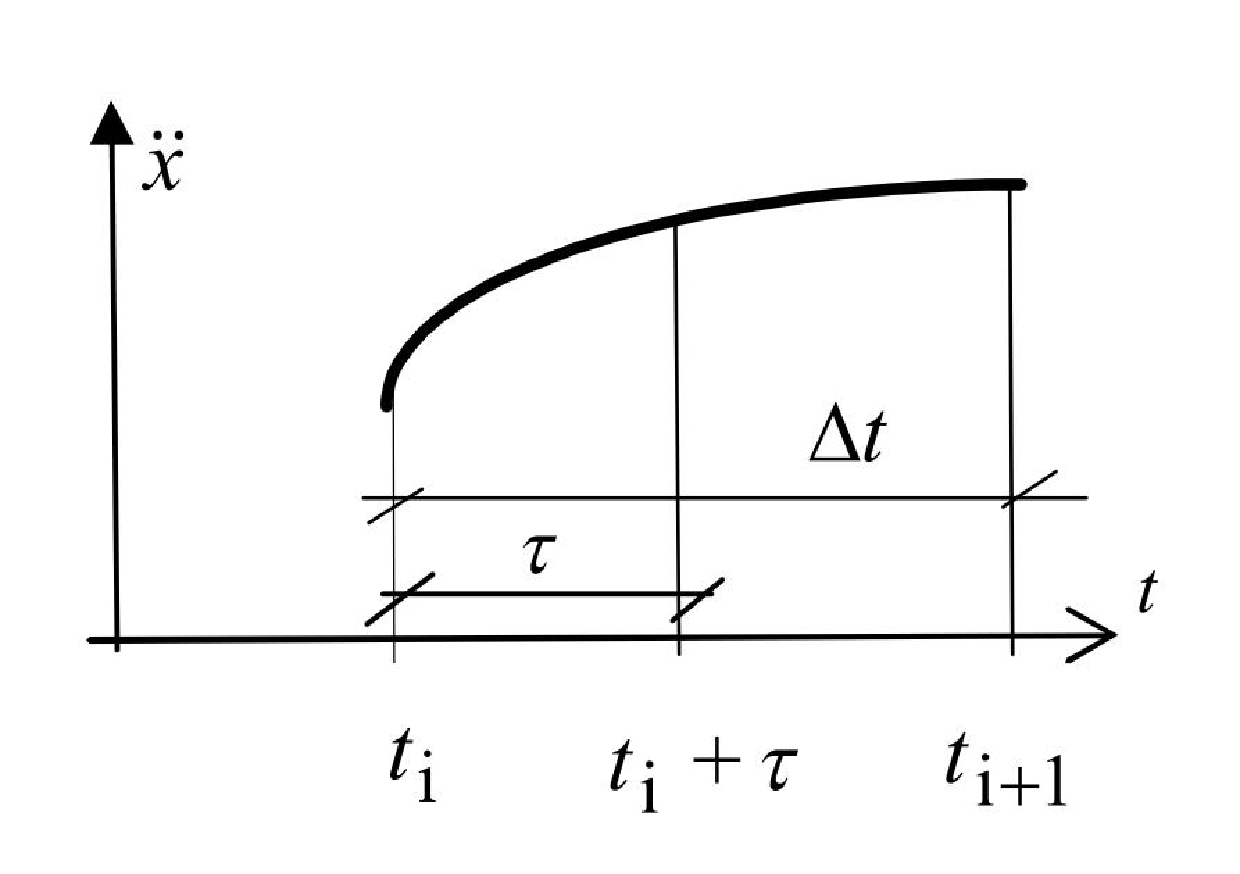
\includegraphics[width=0.45\textwidth]{newmark.pdf}
\caption{A Newmark eljárásnál feltételezett gyorsulás \cite{gyorgyi}.}
\label{fig:newmark}
\end{figure}

Az eljárás implicit, mivel a \eqref{newmark2} egyenlet alapján az i+1-dik  időpontbeli elmozdulás meghatározásához az i+1-dik  időpontbeli gyorsulásra is szükség van.

A $\gamma$ és $\beta$ paraméterek értékétől függően megkülönböztetünk néhány speciális esetet\cite{chopra,crcontthe}. Ha $(\gamma,\beta)=(1/2,1/4)$, akkor két időlépés között a gyorsulás konstans, és az átlagos értékkel egyezik meg, $(\gamma,\beta)=(1/2,1/6)$ értékpár esetén pedig lineáris a gyorsulás. A $(\gamma,\beta)=(1/2,0)$ esetet explicit Newmark eljárásnak nevezzük.

\begin{figure}[h!]
\centering
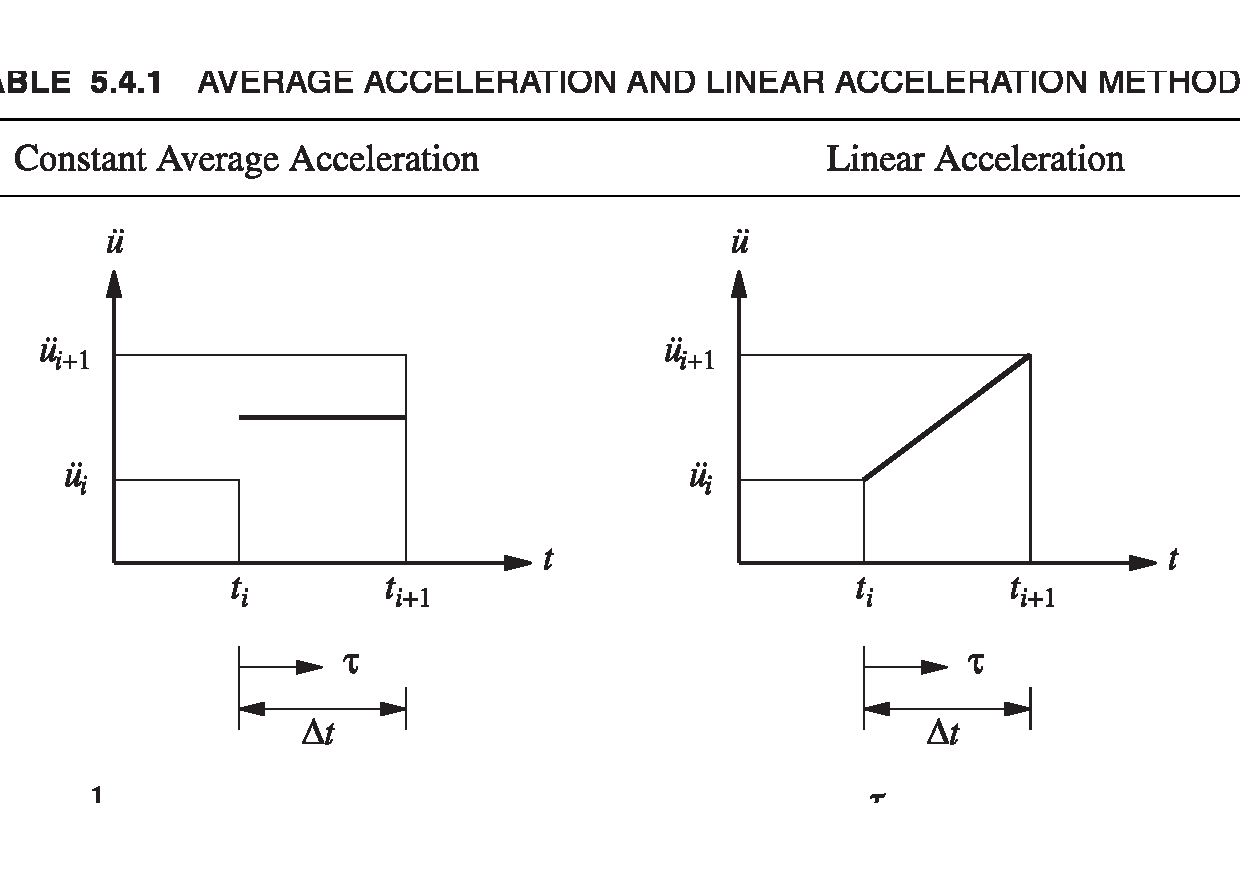
\includegraphics[trim = 0mm 15mm 0mm 20mm, clip, width=\textwidth]{newmark_spec.pdf}
\caption[Konstans átlagos gyorsulás és lineáris gyorsulás feltételezése]{Konstans átlagos gyorsulás (Constant Average Acceleration) és lineáris gyorsulás (Linear Acceleration) feltételezése \cite{chopra}.}
\label{fig:newmark spec}
\end{figure}

Az eljárás stabilitása és pontossága a $\gamma$ és $\beta$ paraméterek függvénye \cite{chopra}. A stabilitás feltétele tetszőleges $\gamma$-ra és $\beta$-ra a következő egyenlet teljesülése:
\begin{equation*}
\frac{\Delta{t}}{T_m}\leq\frac{1}{\pi\sqrt{2}}\frac{1}{\sqrt{\gamma-2\beta}}.
\end{equation*}
 Az eljárás feltétel nélkül stabil, ha
\begin{equation*}
\gamma\geq\frac{1}{2}, \qquad \beta\geq\frac{1}{4}\left(\frac{1}{2}+\gamma\right)^2, 
\end{equation*}
mivel a feltétel ekkor
\begin{equation*}
\frac{\Delta{t}}{T_m}<\infty.
\end{equation*}
Lineáris gyorsulás esetén  az egyenlőtlenségbe behelyettesítve
\begin{equation*}
\frac{\Delta{t}}{T_m}\leq0.551 
\end{equation*}
feltétel adódik az időlépés nagyságára, azonban ennél az eljárás pontossága érdekében a korábban ismertetett \eqref{dt max} képlet alapján kisebb lépésközt érdemes használni.

\subsection{Hilbert-Hughes-Taylor módszer}

{\ }

A Hilbert-Hughes-Taylor (továbbiakban HHT-$\alpha$ \cite{hht, hht_wiki}) módszer a Newmark eljárás módosítása. Alapja a Newmark eljárásnál definiált \eqref{newmark1} és \eqref{newmark2} egyenlet - $\gamma$ és $\beta$ paraméterek ugyanazzal a jelentéssel bírnak -, de a \eqref{rezgegyi+1} egyenlet helyett az alábbi egyenletbe helyettesítünk:
\begin{equation}
\mathbf{M}\mathbf{\ddot{u}}_{i+1}+\alpha\mathbf{C}\mathbf{\dot{u}}_{i+1}+(1-\alpha)\mathbf{C}\mathbf{\dot{u}}_{i}+\alpha\mathbf{K}\mathbf{u}_{i+1}+(1-\alpha)\mathbf{K}\mathbf{u}_i=\mathbf{q}_{i+\alpha},
\end{equation}
tehát a \eqref{rezgesegy} egyenletet a $t_{i+\alpha} = (i+\alpha)\Delta{t}$ időpillanatban elégítjük ki.
Ekkor a \eqref{newmark long} egyenlet a következőképpen módosul:
\begin{equation}
\label{hht long}
\begin{split}
\left(\alpha\mathbf{K}+\frac{1}{\beta\Delta{t}^2}\mathbf{M}+\frac{\gamma}{\beta\Delta{t}}\alpha\mathbf{C}\right)\mathbf{u}_{i+1} = \mathbf{q}_{i+\alpha}+\mathbf{M}\left[\frac{1}{\beta\Delta{t}^2}\left(\mathbf{u}_i+\mathbf{\dot{u}}_i\Delta{t}\right)+\left( \frac{1}{2\beta}-1\right)\mathbf{\ddot{u}}_i\right]        \\ +\alpha\mathbf{C}\left[\frac{\gamma}{\beta\Delta{t}}\mathbf{u}_i+\left(\frac{\gamma}{\beta}-1\right)\mathbf{\dot{u}}_i+\left(\frac{\gamma}{2\beta}-1\right)\Delta{t}\mathbf{\ddot{u}}_i\right]-(1-\alpha)\mathbf{C}\mathbf{\dot{u}}_i-(1-\alpha)\mathbf{K}\mathbf{u}_i,
\end{split}
\end{equation}
ahol
\begin{equation*}
\mathbf{q}_{i+\alpha} = \mathbf{q}(t_i+\alpha\Delta{t}).
\end{equation*}
%
Rövidebb alakban:
\begin{equation}
\label{hht short}
\mathbf{\hat{K}}_{\alpha}\mathbf{u}_{i+1} = \mathbf{\hat{q}}_{i+\alpha},
\end{equation}
ahol $\mathbf{\hat{K}}$ a hatékony merevségi mátrix, $\mathbf{\hat{q}}_{i+\alpha}$ pedig a hatékony tehervektor a $t_{i+\alpha}$ időpillanatban.


A módszer a Newmark eljáráshoz hasonlóan implicit. A stabilitás és pontosság a HHT-$\alpha$ módszernél is az integrálási paraméterektől függ, azonban $\gamma$ és $\beta$ függvénye $\alpha$-nak, melynek értéke $0.67$ és $1.00$ között változhat. Minél kisebb $\alpha$ értéke, annál pontosabb a módszer. Az $\alpha=1.0$ eset a Newmark eljárással egyezik meg. A módszer feltétel nélkül stabil, ha
\begin{equation*}
\beta = \frac{(2-\alpha)^2}{4}, \qquad \gamma = \frac{3}{2}-\alpha
 \end{equation*}

\subsection{Wilson-$\boldsymbol\theta$ eljárás}

{\ }

Az eljárás a $t$ és $t+\theta\Delta{t}$ időpontok között lineáris gyorsulásváltozást tételez fel, és szintén $t+\Delta{t}$ időpontban számítja az elmozdulást. A $\theta$ paraméternek az eljárás stabilitásában van szerepe.
A lineáris gyorsulásváltozás alapján egy $t+\tau$ időpontban felírhatók a gyorsulásvektorra, valamint a vektor integrálásával a sebességvektorra és az elmozdulásvektorra  vonatkozó összefüggések:
\begin{subequations}
\begin{align}
\mathbf{\ddot{u}}_{t+\tau} & = \mathbf{\ddot{u}}_{t}+\frac{\tau}{\theta\Delta{t}}\left(\mathbf{\ddot{u}}_{t+\theta\Delta{t}}-\mathbf{\ddot{u}}_t\right), \label{wilson_tau1}\\
\mathbf{\dot{u}}_{t+\tau} & = \mathbf{\dot{u}}_t+\mathbf{\ddot{u}}_t\tau+\frac{1}{2}\frac{\tau^2}{\theta\Delta{t}}\left(\mathbf{\ddot{u}}_{t+\theta\Delta{t}}-\mathbf{\ddot{u}}_t\right), \label{wilson_tau2}\\
\mathbf{u}_{t+\tau} & = \mathbf{u}_t+\mathbf{\dot{u}}_t\tau+\frac{1}{2}\mathbf{\ddot{u}}_t\tau^2+\frac{1}{6}\frac{\tau^3}{\theta\Delta{t}}\left(\mathbf{\ddot{u}}_{t+\theta\Delta{t}}-\mathbf{\ddot{u}}_t\right).\label{wilson_tau3}
\end{align}
\end{subequations}
A gyorsulásvektor és sebességvektor a $t+\theta\Delta{t}$ időpontban kifejezve:  
\begin{subequations}
\begin{align}
\mathbf{\ddot{u}}_{t+\theta\Delta{t}} & = \frac{6}{(\theta\Delta{t})^2}\left(\mathbf{u}_{t+\theta\Delta{t}}-\mathbf{u}_t\right)-\frac{6}{\theta\Delta{t}}\mathbf{\dot{u}}_t-2\mathbf{\ddot{u}}_t, \label{wilson theta a}\\
\mathbf{\dot{u}}_{t+\theta\Delta{t}} & = \frac{3}{\theta\Delta{t}}\left(\mathbf{u}_{t+\theta\Delta{t}}-\mathbf{u}_t\right)-2\mathbf{\dot{u}}_t-\frac{\theta\Delta{t}}{2} \mathbf{\ddot{u}}_t. \label{wilson theta v}
\end{align}
\end{subequations}
%
Mivel a gyorsulást lineárisnak feltételezzük $t$ és $t+\theta\Delta{t}$ időpontok között, az erőváltozást is lineárisnak kell tekintenünk. A $t+\theta\Delta{t}$ időponthoz tartozó erő:
\begin{equation*}
\mathbf{q}_{t+\theta\Delta{t}} = \mathbf{q}_t+\theta\left(\mathbf{q}_{t+\Delta{t}}-\mathbf{q}_t\right). 
\end{equation*}
Az \eqref{rezgesegy} alatti mátrix-differenciálegyenletet a $t+\theta\Delta{t}$ időpontra felírva $\mathbf{u}_{t+\theta\Delta{t}}$-re az alábbi egyenletet kapjuk:
\begin{equation}
\begin{split}
\label{wilson long}
\left(\mathbf{K}+\frac{3}{\theta\Delta{t}}\mathbf{C}+\frac{6}{(\theta\Delta{t})^2}\mathbf{M}\right)\mathbf{u}_{t+\theta\Delta{t}} = \mathbf{q}_t+\theta\left(\mathbf{q}_{t+\Delta{t}}-\mathbf{q}_t\right)\\+\mathbf{M}\left(\frac{6}{(\theta\Delta{t})^2}\mathbf{u}_t+\frac{6}{\theta\Delta{t}}\mathbf{\dot{u}}_t+2\mathbf{\ddot{u}}_t\right)+\mathbf{C}\left(\frac{3}{\theta\Delta{t}}\mathbf{u}_t+2\mathbf{\dot{u}}_t+\frac{\theta\Delta{t}}{2} \mathbf{\ddot{u}}_t\right).
\end{split}
\end{equation}
Rövidebb alakban felírva az egyenletet:
\begin{equation}
\label{wilson short}
\mathbf{\hat{K}}_{\theta}\mathbf{u}_{t+\theta\Delta{t}} = \mathbf{\hat{q}}_{t+\theta\Delta{t}},
\end{equation}
ahol  $\mathbf{\hat{K}}$ a hatékony merevségi mátrix, $\mathbf{\hat{q}}_{t+\theta\Delta{t}}$ pedig a hatékony tehervektor a $t_{i+\theta}$ időpillanatban. Az együtthatómátrix lineáris esetben időfüggetlen, tehát a számítások során elég egyszer előállítani és invertálni. Az eljárás implicit, mivel az elmozdulás a $t+\Delta{t}$ időpontban  függ a $t+\Delta{t}$ időpontban meghatározott erőtől.

Az $\mathbf{u}_{t+\theta\Delta{t}}$ ismeretében $\mathbf{\ddot{u}}_{t+\theta\Delta{t}}$ meghatározható a \eqref{wilson theta a} képlettel. Az $\mathbf{\ddot{u}}_{t+\theta\Delta{t}}$ valamint $t+\tau = t+\theta\Delta{t}$  a \eqref{wilson_tau1}, \eqref{wilson_tau2} és \eqref{wilson_tau3} képletekbe való behelyettesítésével számíthatjuk az $\mathbf{\ddot{u}}_{t+\Delta{t}}$, $\mathbf{\dot{u}}_{t+\Delta{t}}$ és az $\mathbf{u}_{t+\Delta{t}}$ vektorokat.

A eljárás feltétel nélküli stabilitása $\theta>1.37$ paraméter esetén biztosítható. A periódusidő meghosszabbodása függ az integrálási lépésköztől és a $\theta$ paramétertől, ennek optimális értéke  $1.40$.


\subsection{Chen-Ricles algoritmus}\label{subsec:cr}

{\ }

A Chen-Ricles (továbbiakban CR \cite{crcontthe}) algoritmus szintén a Newmark eljárásnál a \eqref{newmark1} és \eqref{newmark2} pontban ismertetett egyenletekből indul ki. Az eljárást elsősorban hibrid szimulációs módszerhez fejlesztették ki, de az algoritmus használható önálló numerikus számításként is. A sebességvektort és az elmozdulásvektort a következő összefüggések alapján számolja:  
\begin{subequations}
\begin{align}
\mathbf{\dot{u}}_{i+1} & = \mathbf{\dot{u}}_i+\boldsymbol\alpha_1\Delta{t}\mathbf{\ddot{u}}_i, \\
\mathbf{u}_{i+1} & = \mathbf{u}_i+\Delta{t}\mathbf{\dot{u}}_{i}+\boldsymbol\alpha_2\Delta{t}^2\mathbf{\ddot{u}}_i.
\end{align}
\end{subequations}
 Ezeket behelyettesítve a \eqref{rezgegyi+1} egyenletbe számítható a gyorsulásvektor. Az $\mathbf{\dot{u}}_{i+1}$ és $\mathbf{u}_{i+1}$ vektorok csak az $i$-dik időlépésben számolt értékektől függnek, tehát az eljárás explicit. A $t_{i+1}$ időpontbeli gyorsulást a \eqref{rezgegyi+1}  mozgásegyenletből számíthatjuk, $\mathbf{\dot{u}}_{i+1}$ és $\mathbf{u}_{i+1}$ vektorok behelyettesítésével:
\begin{equation}
\mathbf{\ddot{u}}_{i+1} = \mathbf{M}^{-1}(\mathbf{q}_{i+1}-\mathbf{C}\mathbf{\dot{u}}_{i+1}-\mathbf{K}\mathbf{u}_{i+1})
\end{equation} 
  
A módszer stabilitása a legtöbb explicit eljárással ellentétben frekvenciafüggetlen, azaz feltétel nélküli, ha  $\boldsymbol\alpha_1$ és  $\boldsymbol\alpha_2$ értékére teljesül a következő:
\begin{equation}
\label{cr alpha}
\boldsymbol\alpha_1 = \boldsymbol\alpha_2 = 4(4\mathbf{M}+2\Delta{t}\mathbf{C}+\Delta{t}^2\mathbf{K})^{-1}\mathbf{M}.
\end{equation}
Lineáris esetben a \eqref{cr alpha} mátrix időfüggetlen, ezért  előállítását elég egyszer elvégezni.


\section {Időlépéses módszerek alkalmazása nemlineáris rendszerek vizsgálatára}\label{sec:nl idolepmsz}

{\ }

A legtöbb építőmérnöki szerkezet nem csak lineárisan viselkedő elemeket tartalmaz, így viselkedésük leírására nem alkalmazhatók a hagyományos lineáris eljárások. Ilyenkor nemlineáris modellek segítségével sokkal pontosabb számításokat végezhetünk, ezáltal gazdaságosabb, jobban kihasznált szerkezeteket hozhatunk létre. Azonban a nemlineáris számítási módszerek sokkal bonyolultabbak, nehezebben programozhatók, és  a számítás hosszadalmasabb. 

A nemlineáris számításokra \cite{molnar} leggyakrabban a következők miatt lehet szükség:
\begin{itemize}
\item[--] a  felhasznált anyagok viselkedéséből adódó anyagi nemlinearitás (képlékenyedés: keményedés vagy 
lágyulás),
\item[--]  a szerkezet nagy alakváltozásai miatt létrejövő geometriai nemlinearitás hatása,
\item[--]  a szerkezet elmozdulásai miatt  módosuló  támaszrendszer hatása (peremfeltételi 
nemlinearitás).
\end{itemize}
Ezek viszonylag gyakran fordulnak elő az építőmérnöki gyakorlatban. A szerkezetek gazdaságossága miatt  például sokszor alkalmazunk olyan elemeket, amiknek kihasználjuk a képlékeny tartalékait is, a módosult támaszrendszer és a geometriai nemlinearitás kialakulása pedig fennáll a nagyobb dinamikus terhelések esetén, mint például a szélterhelés vagy a szeizmikus terhelés.

A nemlineáris számításokra vizsgált problémától függetlenül igaz, hogy a kiindulási feltételek jelentősen befolyásolják a vizsgálat eredményét, hogy nem alkalmazhatjuk a szuperpozíció elvét, és az, hogy  a teljes terheléstörténetet figyelembe kell vennünk. Ez utóbbi a dinamikus mozgásegyenletek esetében azt jelenti, hogy a $\mathbf{K}\mathbf{u}$ szorzat helyett egy elmozdulástól függő visszatérítő erőt használunk, amit minden időlépésben újra kell számolni. Ez sok esetben azt jelenti, hogy a megoldás együttható mátrixát minden időlépésben újra elő kell állítani és invertálni, ami elég hosszadalmas nagy szerkezetek esetében.

A rugalmas visszatérítő erő függvényének megválasztása a rendszerben alkalmazott nemlineáris anyagmodell alapján nehéz feladat, mert dinamikus terhelésre nem ismerünk jelenleg kellően pontos nemlineáris anyagmodellt. A visszatérítő erő számítása az egyes megoldási módszereknél lehet explicit, amikor  az $\mathbf{f}_{s,i}$ az $\mathbf{u}_i$-től függő mennyiség, illetve implicit, amikor az $\mathbf{f}_{s,i+1}$ az ismeretlen $\mathbf{u}_{i+1}$ függvénye. 

Nagyméretű szerkezetek vizsgálatánál a számítási sebesség szempontjából különösen fontos, hogy az explicit módszereknél kisebb időlépésköz használható az implicit eljárásokhoz képest. Viszont az implicit módszereknél, bár nagyobb időlépésköz a megengedett, és a szerkezet könnyebben kezelhető,  minden időlépésben iterációval közelítjük a megoldást. Az iterációk  számának  növelésével  javítható  az  eredmény  pontossága, azonban ez növeli a számításhoz szükséges időintervallumot is. Számítógépes programokban legtöbbször az implicit módszereket alkalmazzák. A következőkben a két legelterjedtebb módszernek, a centrális differenciák módszerének és a Newmark eljárásnak nemlineáris feladatokra való alkalmazását mutatom be.  





\subsection{Centrális differenciák módszere}

{\ }

A nemlineáris centrális differenciák módszerénél \cite{chopra} az elmozdulásvektorok függvényét a $t_{i-1}, t_i$ és $t_{i+1}$ időpontok között továbbra is  másodfokú parabolákkal közelítjük.

\begin{align*}
\label{centdiff_av}
\mathbf{\dot{u}}_i&=\frac{1}{2\Delta{t}}\left(\mathbf{u}_{i+1}-\mathbf{u}_{i-1}\right), \\
\mathbf{\ddot{u}}_i&=\frac{1}{\Delta{t}^2}\left(\mathbf{u}_{i+1}-2\mathbf{u}_i+\mathbf{u}_{i-1}\right).
\end{align*}
Az elmozdulásvektor pedig a következő alakban írható fel:
\begin{equation}
\mathbf{u}_{i+1} = \mathbf{u}_i+\Delta{\mathbf{u}}_i.
\end{equation}
A differenciahányadosokat behelyettesítve a \eqref{rezgegyi_nl} alatti mátrix-differenciálegyenletbe $\Delta{\mathbf{u}}_{i}$-re az alábbi összefüggést kapjuk:
\begin{equation}
\label{centdiff_nl}
\left(\frac{1}{\Delta{t}^2}\mathbf{M}+\frac{1}{2\Delta{t}}\mathbf{C}\right)\Delta{\mathbf{u}}_{i} = \mathbf{q}_i-\mathbf{f}_{s,i}+\left(\frac{1}{\Delta{t}^2}\mathbf{M}-\frac{1}{2\Delta{t}}\mathbf{C}\right)\Delta{\mathbf{u}}_{i-1}.
\end{equation}
Ezt szintén felírhatjuk rövidebb alakban:
\begin{equation}
\mathbf{\hat{M}}\Delta{\mathbf{u}}_i = \mathbf{\hat{q}}_i,
\end{equation}
ahol $\mathbf{\hat{M}}$ a hatékony tömegmátrix, $\mathbf{\hat{q}}_i$ pedig a hatékony tehervektor $t_i$ időpillanatban. A lineáris \eqref{centdiff long} és \eqref{centdiff short} egyenletekkel összehasonlítva az egyetlen különbség a $\mathbf{\hat{q}}_i$ vektorban található. 

Az $\mathbf{f}_{s,i}$ visszatérítő erő explicit módon származtatható a $t_i$ időpontbeli válaszból. Az együtthatómátrixban  nem szerepel a visszatérítő erő, ezért a vizsgálat ideje alatt állandó, és így elég azt  egyszer előállítani és invertálni, így az iteratív  nemlineáris eljárásokhoz képest a centrális differenciák módszere sokkal gyorsabb számítást tesz lehetővé. Ezáltal a módszer a legegyszerűbb nemlineáris eljárásnak tekinthető, viszont a többi eljáráshoz képest kevésbé pontos, ezért pontosabb számítást igénylő feladatokhoz általában nem ezt alkalmazzák.


\subsection{Statikus nemlineáris vizsgálat Newton-Raphson iteráció segítségével}

{\ }

 Implicit módszereknél, mint a Newmark eljárás, általában a kvázi-Newton-Raphson iterációs módszert \cite{chopra} használjuk a visszatérítő erő meghatározására, így a számítás nagy rendszereknél sokkal több időt vesz igénybe. A következőkben ismertetem a Newton-Raphson  iterációs eljárást statikus nemlineáris szerkezetek vizsgálatára.

A tehetetlenségi és csillapítási tulajdonságok elhanyagolásával a nemlineáris mozgásegyenlet a következő statikus problémaként írható fel:

\begin{equation*}
\mathbf{f}_s(\mathbf{u}) = \mathbf{q}.
\end{equation*}
Tehát a feladat a külső erőből adódó  elmozdulások meghatározása, úgy, hogy a erő és az elmozdulás kapcsolata, az $\mathbf{f}_s(\mathbf{u})$ visszatérítő erő függvény ismert a vizsgált rendszerben. A megoldáshoz iterációs eljárást alkalmazunk. Az iteráció $j$-edik lépésének elején  az ismert $\mathbf{u}^j$-ből számítható a kiegyensúlyozatlan erő:
\begin{equation*}
\mathbf{R} = \mathbf{q}-\mathbf{f}_s(\mathbf{u}^j)
\end{equation*}
 A visszatérítő erőt a   Taylor-sorba fejtjük a Newton-Raphson iteráció $j$-edik lépésében meghatározott $\mathbf{u}^j$ körül, majd a magasabbrendű tagokat elhanyagolva:
\begin{equation}
\label{f_s^j+1}
\mathbf{f}_s^{(j+1)} = \mathbf{f}_s^{(j)}+\mathbf{K}_T^{(j)}\Delta{\mathbf{u}}^{(j)} = \mathbf{q},
\end{equation}
ahol 
\begin{equation*}
\mathbf{K}_T^{(j)} = \left. \frac{\delta\mathbf{f}_s}{\delta\mathbf{u}} \right|_{\mathbf{u}^{(j)}},
\end{equation*}
az érintőmerevség mátrixa a visszatérítő erő $\mathbf{u}$ szerinti deriváltja az $\mathbf{u}^{(j)}$ helyen számítva, és $\Delta{\mathbf{u}}^{(j)} = \mathbf{u}^{(j+1)}-\mathbf{u}^{(j)}$  két egymást követő iteráció különbsége.

A \eqref{f_s^j+1} egyenletet megoldva megkapjuk  $\Delta{\mathbf{u}}^{(j)}$-t, ennek segítségével számíthatjuk $\mathbf{u}^{(j+1)}$ értékét.
%
\begin{equation}
\label{NR_u_j+1}
\mathbf{u}^{(j+1)} = \mathbf{u}^{(j)}+\Delta{\mathbf{u}}^{(j)} =  \mathbf{u}^{(j)}+\mathbf{K}_T^{(j)-1}(\mathbf{q}-\mathbf{f}_s^{(j)})
\end{equation}
Ezt tetszőleges iterációs lépésen keresztül számíthatjuk, az eredmények $\mathbf{u}$-hoz konvergálnak.  A gyorsabb konvergencia érdekében  a $\mathbf{q}$ terhet  $k$ darab $\Delta{\mathbf{q}}$ nagyságú teherlépcsőben szokták felvinni, ilyenkor egy-egy iteráció egy $\mathbf{u}_k$-hoz tart.

A módosított, kvázi-Newton-Raphson módszer abban különbözik az előbb leírtaktól, hogy a $\mathbf{K}_T$ érintőmerevséget nem számítjuk minden egyes  lépésben, csak teherlépcsőnként egyszer. A $k$-adik teherlépcsőn az $\mathbf{u}_{k}$ elmozduláshoz számított értékével vesszük figyelembe. Ennek eredményeképp a számítás sokkal egyszerűbb és gyorsabb, viszont a konvergencia lassabb lesz.

A megoldást minden iteráció után ellenőrizni kell, és ha valamelyik mennyiség eltérése egy hibahatáron belülre kerül, az iterációt nem érdemes tovább folytatni. Általában ennek ellenőrzésére a következő konvergenciakritériumokat használják:
\begin{itemize}
\item a maradék kiegyensúlyozatlan erő kisebb az előírtnál:
\begin{equation*}
\parallel \mathbf{R}^{(j)} \parallel \leq \epsilon_R
\end{equation*}
\item az elmozdulás változása kisebb az előírt értéknél:
\begin{equation*}
\parallel \Delta{\mathbf{u}}^{(j)} \parallel \leq \epsilon_u
\end{equation*}
\item az elmozdulásváltozást előidéző maradék kiegyensúlyozatlan erő által végzett munka kisebb az előírtnál:
\begin{equation*}
\frac{1}{2}\parallel \Delta{\mathbf{u}}^{(j)}\mathbf{R}^{(j)} \parallel \leq \epsilon_w
\end{equation*}
\end{itemize}

\subsection{Newmark eljárás}

{\ }

A  lineáris eljárásnál bemutatott \eqref{newmark1} és \eqref{newmark2} egyenletek továbbra is érvényesek:
%
\begin{align*}
\mathbf{\dot{u}}_{i+1}& =  \mathbf{\dot{u}}_i+[(1-\gamma)\Delta{t}]\mathbf{\ddot{u}}_i+(\gamma\Delta{t})\mathbf{\ddot{u}}_{i+1},   \\ 
\mathbf{u}_{i+1}& =  \mathbf{u}_i+\Delta{t}\mathbf{\dot{u}}_i+\left[(0.5-\beta)
(\Delta{t})^2\right]\mathbf{\ddot{u}}_i+\left[\beta(\Delta{t})^2\right]\mathbf{\ddot{u}}_{i+1}. 
\end{align*}
%
A nemlineáris Newmark eljárásnál \cite{chopra} a nemlineáris statikus vizsgálatnál bemutatott kvázi-Newton-Raphson iterációs módszert alkalmazzuk, azonban az eljárás során nem hanyagolhatjuk el a tehetetlenségi és csillapító tagokat.  Jelölje $\mathbf{\hat{f}}_{s,i+1}$ az $i$-edik időlépés $j$-edik iterációjában számított hatékony visszatérítő erőt. Ekkor:
%
\begin{equation*}
 \mathbf{\hat{f}}_{s,i+1} = \mathbf{M}\mathbf{\ddot{u}}_{i+1}+\mathbf{C}\mathbf{\dot{u}}_{i+1}+\mathbf{f}_{s,i+1} = \mathbf{q}_{i+1}.
\end{equation*}
 % 
 Az $\mathbf{\hat{f}}_{s,i+1}^{(j+1)}$ hatékony visszatérítő erő Taylor sorba fejtését elvégezve, az első két tag figyelembevételével a \eqref{f_s^j+1}   egyenlettel összeegyeztethető alakúra hozható a megoldás:
 %
 \begin{equation}
\label{Newmark_f_s^j+1}
\mathbf{\hat{f}}_{s,i+1}^{(j+1)} = \mathbf{f}_{s,i+1}^{(j)}+\mathbf{\hat{K}}_{T,i+1}\Delta{\mathbf{u}}^{(j)} = \mathbf{q}_{i+1},
\end{equation}
ahol
\begin{equation*}
\mathbf{\hat{K}}_{T,i+1} = \frac{\delta\mathbf{\hat{f}}_s}{\delta\mathbf{u}_{i+1}} = \frac{1}{\beta\Delta{t}^2}\mathbf{M}+\frac{\gamma}{\beta\Delta{t}}\mathbf{C}+\mathbf{K}_{T,i+1},
\end{equation*}
vagyis a hatékony érintőmerevség mátrixa a visszatérítő erő $\mathbf{u}_{i+1}$ szerinti deriváltja, és $\Delta{\mathbf{u}}^{(j)} = \mathbf{u}_{i+1}^{(j+1)}-\mathbf{u}_{i+1}^{(j)}$  két egymást követő iteráció különbsége.  

A \eqref{Newmark_f_s^j+1} egyenletet megoldva az egyes iterációs lépéseknél  megkapjuk $\Delta{\mathbf{u}}^{(j)}$-t, ennek segítségével számíthatjuk $\mathbf{u}_{i+1}^{(j+1)}$ értékét.
%
\begin{equation}
\label{Newmark_u_j+1}
\mathbf{u}_{i+1}^{(j+1)} = \mathbf{u}_{i+1}^{(j)}+\Delta{\mathbf{u}}^{(j)} =  \mathbf{u}_{i+1}^{(j)}+\mathbf{\hat{K}}_{T,i+1}^{-1}(\mathbf{q}_{i+1}-\mathbf{\hat{f}}_{s,i+1}^{(j)})
\end{equation}

Egy másik megközelítés alapján a gyorsulást fejezzük ki  a mozgásegyenletből. (A \ref{sec: nemlin progi} pontban bemutatásra kerülő nemlineáris megoldóprogramban mindkét megközelítés algoritmusa szerepel.)
\begin{equation}
\begin{split}
\left( \mathbf{M}+\Delta{t}\gamma\mathbf{C}+\Delta{t}^2\beta\mathbf{K}_{T,i+1}\right)\mathbf{\ddot{u}}_{i+1}^{(j+1)} = \mathbf{q}_{i+1} + \mathbf{r}_{i+1}^{(j)}-\mathbf{f}_{s,i+1}^{(j)}\\-\left(\mathbf{u}_i^{(j)}+\Delta{t}(1-\gamma)\mathbf{\ddot{u}}_i^{(j)}\right)\mathbf{C}-\left(\Delta{t}\mathbf{\dot{u}}_i^{(j)}+(0,5-\beta)\Delta{t}^2\mathbf{\ddot{u}}_i^{(j)}\right)\mathbf{K}_{T,i+1},
\end{split}
\end{equation}
ahol $\mathbf{r}_{i+1}^{(j)}$ a $j$-edik iterációnál keletkező, még kiegyensúlyozatlan erő. Az egyes iterációs lépésekben $\mathbf{u}_i^{(j)}$ elmozdulás- és $\mathbf{\dot{u}}_i^{(j)}$ sebességvektorokat a \eqref{newmark1} és \eqref{newmark2} egyenletekből, az $\mathbf{f}_{s,i+1}^{(j)}$ visszatérítő erőt pedig  $\mathbf{u}_i^{(j)}$ elmozdulásvektorból számíthatjuk.

Látható, hogy a nemlineáris Newmark eljárás a nemlineáris centrális differenciák módszeréhez képest sokkal bonyolultabb, és az iterációs számítás nagy rendszerek esetében jelentősen hosszabb. Viszont az eljárás előnyei közé tartozik, hogy feltétel nélkül stabil a \ref{subsec:Newmark_lin} pontban ismertetett integráló paraméterértékek esetén, illetve hogy  sokkal  pontosabb megoldásokkal szolgál, mint a centrális differenciák módszere. A Newmark eljárást sokszor alkalmazzák nemlineáris problémák megoldására.



\section{Az időlépéses módszerek alkalmazása}

{\ }

A tárgyalt lineáris és nemlineáris integráló formulákat a különböző, numerikus számításokat végző  programok használják közönséges differenciálegyenletek kezdetiérték feladatainak megoldására.  Különböző alkalmazási területeken más-más módszerek preferáltak. A legtöbbször a hagyományos eljárásokat, mint például  az Euler és a Runge-Kutta módszereket, illetve az építőmérnöki gyakorlatban a Newmark eljárást alkalmazzák.

Az általános matematikai számításokra használt szoftverek, mint például a MATLAB, a Maple vagy a Wolfram Mathematica általában a klasszikus formulákat alkalmazzák. Ezek vagy az utasításkészletbe beépített  függvényként találhatók, vagy könnyen beprogramozhatók. Léteznek a numerikus integráló formulákat tartalmazó függvénykönyvtárak is, amelyeket más programokban is lehet használni. A MATLAB programrendszerben az Ode rutinok alkalmazhatók közönséges differenciálegyenletek megoldására. Ezek között találhatók olyan egyszerűbb  módszerek, mint az Euler-Cauchy vagy a Runge-Kutta, vagy kicsivel bonyolultabb módszerek is, mint a beágyazott Runge-Kutta módszerek. Az Ode45 rutin például egy egylépéses, váltakozó lépésközű  beágyazott Runge-Kutta módszer, ami kiszámol egy negyed- és egy ötödrendű Runge-Kutta módszert, és úgy számol lépésközt, hogy a hiba a negyedrendű módszer hibája legyen. Az Ode megoldók nevében a számok sokszor azt jelzik, hogy hányad rendű módszereket alkalmaznak. 

A mérnöki gyakorlatban használt végeselemes programok általában vagy egy egyszerűbb explicit formulát alkalmaznak mint a centrális differenciák módszere, vagy egy pontosabb implicit formulát használnak, mint a Newmark eljárás. A centrális differenciák módszerét alkalmazzák például az LS/DYNA és az ABAQUS/Explicit szoftverek \cite{chopra}. Az explicit módszerek általában nem praktikusak nagyméretű szerkezetek elemzésére, mert  kisebb időlépések alkalmazását igénylik, viszont nagy előnyük, hogy jól használhatók a párhuzamosan több számítógépen futó számításokra. A végeselemes programok közül  azonban a legtöbb  a Newmark eljárást alkalmazza lineáris és nemlineáris számításokra, ilyen például az ANSYS és az AxisVM programcsomag. A NONSAP szoftver Wilson-$\boldsymbol\theta$ és Newmark eljárást is használ. Az implicit eljárások előnye, hogy nagyobb időlépésköz a megengedett, így a  nagy szerkezetek is könnyebben kezelhetők.

A mérnökszeizmológiai kutatásokhoz fejlesztett   végeselemes  szoftver  az OpenSEES (Open System for Earthquake Engineering Simulation). A programban az összes korábban ismertetett direkt integráló formula kiválasztható a dinamikus számításokhoz.

Az ismertetett integráló formulákat használva lineáris, nemlineáris és hibrid szimulációs programokat fejlesztettem MATLAB szoftver segítségével, melyeket a \ref{chap: lin+nemlin progi}. és a \ref{chap: hibrid progi}. fejezetekben mutatok be. A programokban nem  az Ode rutinokat, hanem saját megoldó algoritmusokat alkalmaztam. Azért döntöttem a MATLAB szoftver  mellett, mert fő jellemzői közé tartozik, hogy gyorsan számol nagy mátrixokkal, és hogy feladatspecifikusan alkalmazható, ezért laboratóriumi számításokhoz könnyen használható.
